\documentclass[11pt]{article}

\usepackage[margin=1in]{geometry}
\usepackage{amsmath}
\usepackage{amssymb}
\usepackage{tikz}
\usetikzlibrary{arrows.meta}

\title{A Displacement Parameterization of Two Triangular Elements}
\author{}
\date{}

\begin{document}
\maketitle

\section{Overview of the Construction and Plots}

The purpose of this construction is to study a pair of triangular elements
with four nodes. The same four current node positions can be connected by
either of two diagonals. We call the topology with diagonal \((x_2,x_3)\)
the \(T_{23}\) topology, and the topology with diagonal \((x_1,x_4)\) the
\(T_{14}\) topology. The main numerical question is whether a state that is
currently represented by one topology should keep that diagonal or flip to
the other one.

The workflow has four separate layers:
\begin{enumerate}
    \item Choose a current nodal state from the parameters \(w\), \(u\), and
          \(v\).
    \item Choose which topology is considered current, and which topology is
          obtained after flipping the diagonal.
    \item Compute energies, stresses, and metric-based reconnection criteria
          on both topologies.
    \item Draw these quantities on the same \((w,\hbox{parameter})\) grid,
          where the second axis is either \(u\) or \(v\).
\end{enumerate}
Keeping these layers separate is important. The parameterization defines only
the four node positions. The topology then decides which two triangles are
formed from those nodes. Energies, stresses, and reconnection regions are
computed only after both choices have been made.

\subsection{From Parameters to Nodes}

The reference state is a square split into two right triangles. In the
canonical current frame we place the shared edge on the horizontal axis,
\[
    x_2=(0,0), \qquad x_3=(L,0).
\]
The parameter \(w\) controls the length of this shared edge by
\[
    L=\sqrt{2}+w.
\]
The parameters \(u\) and \(v\) control horizontal offsets of the two outer
nodes. The resulting \(T_{23}\) element pair is area preserving by
construction: each triangle has area \(1/2\), so the total area is one.
This area preservation belongs to the \(T_{23}\) parameterization itself. If
the same four nodes are reconnected as \(T_{14}\), the flipped triangles need
not each have determinant one.

\subsection{Current and Flipped Topologies}

The default comparison is the first flip,
\[
    T_{23}\longrightarrow T_{14}.
\]
In this case the current energy and stress are computed on the \(T_{23}\)
triangles, while the flipped energy and stress are computed on the \(T_{14}\)
triangles using the same four node positions. The reverse comparison,
\[
    T_{14}\longrightarrow T_{23},
\]
is useful as a diagnostic ``second flip'' mode, but it should be interpreted
carefully because the nodal parameterization was built to preserve the
\(T_{23}\) areas.

\subsection{Energy Difference}

For each grid point the code evaluates the square-conti energy on the current
and flipped topology. The plotted energy difference is
\[
    \Delta E
      =
      E_{\mathrm{flipped}}-E_{\mathrm{current}}.
\]
Thus a positive value means that the flipped topology has larger energy at
that same nodal state. The dashed black reference contour is not a flipping
criterion. It marks the energy level of two triangular elements under a
horizontal simple shear with \(\gamma=0.5\), including the factor \(1/2\) for
each triangle area.

\subsection{Reconnection Regions}

The reconnection regions are drawn on top of the same parameter grid. They
come from two distinct ideas:
\begin{enumerate}
    \item a local metric test based on the selected edge-vector matrix \(G\),
    \item a shared-edge test checking whether the current diagonal is a
          longest edge of both current triangles.
\end{enumerate}
The code can evaluate \(G\) using the two shortest vectors in each triangle,
or using a fixed corner choice. This is why several region plots can be
generated for the same parameter window. A green dashed Delaunay contour is
also drawn separately; it shows where a Delaunay triangulation would switch
diagonal. That contour is a geometric comparison, not the same object as the
\(G\)-based reconnection rule.

\subsection{Stress Difference}

There are two kinds of stress plots, and they should not be confused. For
stress tensor components the code first forms
\[
    \Delta \sigma
      =
      \sigma_{\mathrm{flipped}}-\sigma_{\mathrm{current}},
\]
and then plots components such as \(\Delta\langle\sigma_{11}\rangle\),
\(\Delta\langle\sigma_{12}\rangle\), or
\(\Delta\langle\sigma_{22}\rangle\). The brackets indicate the selected
two-element aggregation: the average of both elements, the first element
alone, or the second element alone.

For scalar stress measures, such as the von Mises stress, the order is
different. The measure is evaluated on each topology first, and only then is
the difference taken:
\[
    \Delta m
      =
      m(\sigma_{\mathrm{flipped}})
      -
      m(\sigma_{\mathrm{current}}).
\]
This means that the von Mises plot shows \(\Delta\sigma_{\mathrm{vM}}\), not
\(\sigma_{\mathrm{vM}}(\Delta\sigma)\). The reference contour in every stress
plot is computed from the same quantity that appears in that heatmap, evaluated
for the \(\gamma=0.5\) simple-shear reference state.

\section{Reference Configuration}

We start from four material nodes forming a unit square,
\[
    X_2=(0,0), \qquad
    X_3=(1,1), \qquad
    X_1=(1,0), \qquad
    X_4=(0,1).
\]
The unflipped topology is the triangulation sharing the material diagonal
\((X_2,X_3)\):
\[
    T_{23}=\{(1,2,3),(2,3,4)\}.
\]
The flipped topology is
\[
    T_{14}=\{(1,2,4),(1,4,3)\}.
\]

A current nodal state is an ordered tuple
\[
    \mathbf{x}=(x_1,x_2,x_3,x_4),
    \qquad
    x_i\in\mathbb{R}^2.
\]
Since only objective quantities are used, rigid translations and rotations may
be removed. We choose the canonical current frame
\[
    x_2=(0,0),
    \qquad
    x_3=(L,0),
    \qquad
    L>0.
\]
The plotting code uses this same canonical frame for the reference vertices:
the material square above is first mapped to the canonical reference nodal
state defined below, and all deformation gradients are computed relative to
that canonical reference state.

\section{Area-Preserving Two-Element States}

We restrict attention to current states where the two unflipped triangles have
unit Jacobian determinant,
\[
    \det F_{123}=1,
    \qquad
    \det F_{234}=1.
\]
With \(x_2\) and \(x_3\) fixed, these two constraints place the remaining
nodes on lines parallel to the shared edge. Thus the admissible current states
can be written as
\[
    x_1=(sL,-1/L),
    \qquad
    x_4=(tL,1/L),
\]
for two scalar tangential parameters \(s\) and \(t\). Together with
\[
    x_2=(0,0),
    \qquad
    x_3=(L,0),
\]
this gives a three-parameter family \((L,s,t)\).

\section{The \(w,u,v\) Parameters}

The reference shared-edge length in the canonical frame is
\[
    L_0=\sqrt{2}.
\]
Instead of using \(L\) directly as a control variable, we introduce
\[
    w=L-L_0,
    \qquad
    L(w)=L_0+w=\sqrt{2}+w.
\]
In the rest of the document we write simply
\[
    L = L(w)
\]
to keep the formulas readable. At the initial state, \(w=0\) gives
\(L=L_0\), but in general the vertical distance from the shared edge to each
outer node is \(1/L\). Because \(x_2=(0,0)\) and \(x_3=(L,0)\), the parameter
\(w\) is the direct change in the shared-edge length:
\[
    w = |x_3-x_2|-\sqrt{2}.
\]

We also replace \(s\) and \(t\) by
\[
    u=s+t-1,
    \qquad
    v=s-t.
\]
Equivalently,
\[
    s=\frac{1+u+v}{2},
    \qquad
    t=\frac{1+u-v}{2}.
\]
The complete nodal state is therefore
\[
    \mathbf{x}(w,u,v)
      = \bigl(x_1(w,u,v),x_2(w,u,v),x_3(w,u,v),x_4(w,u,v)\bigr),
\]
with
\[
    x_2(w,u,v)=(0,0),
    \qquad
    x_3(w,u,v)=(L,0),
\]
\[
    x_1(w,u,v)
      =
      \left(
        \frac{1+u+v}{2}L,
        -\frac{1}{L}
      \right),
\]
\[
    x_4(w,u,v)
      =
      \left(
        \frac{1+u-v}{2}L,
        \frac{1}{L}
      \right).
\]

The reference nodal state is now defined unambiguously as
\[
    \mathbf{x}_0 = \mathbf{x}(0,0,0).
\]
Explicitly,
\[
    x_2^0=(0,0),
    \qquad
    x_3^0=(\sqrt{2},0),
\]
\[
    x_1^0=\left(\frac{\sqrt{2}}{2},-\frac{1}{\sqrt{2}}\right),
    \qquad
    x_4^0=\left(\frac{\sqrt{2}}{2},\frac{1}{\sqrt{2}}\right).
\]

\section{Geometric Meaning}

The parameter \(w\) changes the length of the shared edge. Positive \(w\)
widens the element pair; negative \(w\) shortens it.

The parameter \(u\) is the symmetric tangential displacement. It changes
\(s\) and \(t\) in the same direction:
\[
    s-\frac{1}{2} = \frac{u+v}{2},
    \qquad
    t-\frac{1}{2} = \frac{u-v}{2}.
\]
Thus the horizontal offsets of the two outer nodes from the midpoint
\(L/2\) are
\[
    x_{1,x}-\frac{L}{2}
      = \frac{L}{2}(u+v),
    \qquad
    x_{4,x}-\frac{L}{2}
      = \frac{L}{2}(u-v).
\]
The parameter \(v\) is the antisymmetric tangential displacement. It enters
with opposite signs for the two outer nodes.

\begin{figure}[ht]
    \centering
    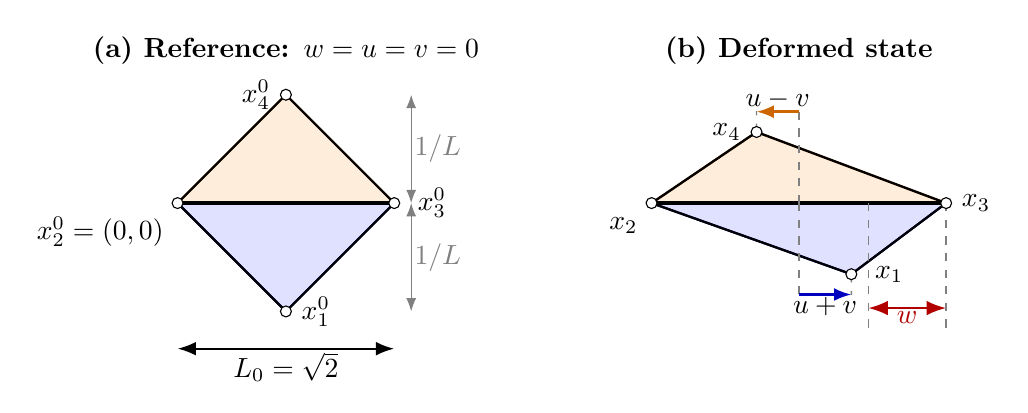
\begin{tikzpicture}[
        scale=0.86,
        >=Latex,
        point/.style={circle,draw=black,fill=white,inner sep=1.4pt},
        triA/.style={fill=blue!12,draw=blue!55!black,line width=0.8pt},
        triB/.style={fill=orange!14,draw=orange!60!black,line width=0.8pt},
        guide/.style={gray,dashed,line width=0.5pt},
        param/.style={-{Latex[length=2.2mm]},line width=0.9pt}
    ]
        \begin{scope}
            \coordinate (r2) at (0,0);
            \coordinate (r3) at (3.2,0);
            \coordinate (r1) at (1.6,-1.6);
            \coordinate (r4) at (1.6,1.6);

            \filldraw[triA] (r1)--(r2)--(r3)--cycle;
            \filldraw[triB] (r2)--(r3)--(r4)--cycle;
            \draw[line width=1.2pt] (r2)--(r3);
            \draw[line width=0.8pt] (r1)--(r2) (r1)--(r3) (r4)--(r2) (r4)--(r3);

            \node[point,label=below left:{$x_2^0=(0,0)$}] at (r2) {};
            \node[point,label={[xshift=0.1cm]right:{$x_3^0$}}] at (r3) {};
            \node[point,label=right:{$x_1^0$}] at (r1) {};
            \node[point,label=left:{$x_4^0$}] at (r4) {};

            \draw[<->,line width=0.8pt] (0,-2.15) -- (3.2,-2.15)
                node[midway,below,fill=white,inner sep=1pt] {$L_0=\sqrt{2}$};
            \draw[<->,gray] (3.45,0) -- (3.45,1.6)
                node[midway,right,fill=white,inner sep=1pt] {$1/L$};
            \draw[<->,gray] (3.45,-1.6) -- (3.45,0)
                node[midway,right,fill=white,inner sep=1pt] {$1/L$};

            \node[font=\bfseries] at (1.6,2.25) {(a) Reference: \(w=u=v=0\)};
        \end{scope}

        \begin{scope}[xshift=7.0cm]
            \coordinate (x2) at (0,0);
            \coordinate (x3ref) at (3.2,0);
            \coordinate (x3) at (4.35,0);
            \coordinate (mid) at (2.175,0);
            \coordinate (x1) at (2.95,-1.05);
            \coordinate (x4) at (1.55,1.05);

            \filldraw[triA] (x1)--(x2)--(x3)--cycle;
            \filldraw[triB] (x2)--(x3)--(x4)--cycle;
            \draw[line width=1.2pt] (x2)--(x3);
            \draw[line width=0.8pt] (x1)--(x2) (x1)--(x3) (x4)--(x2) (x4)--(x3);
            \draw[guide] (mid) -- ++(0,1.55);
            \draw[guide] (mid) -- ++(0,-1.55);
            \draw[guide] (x3ref) -- ++(0,-1.85);
            \draw[guide] (x3) -- ++(0,-1.85);
            \draw[guide] (x1) -- (2.95,-1.55);
            \draw[guide] (x4) -- (1.55,1.55);

            \node[point,label=below left:{$x_2$}] at (x2) {};
            \node[point,label=right:{$x_3$}] at (x3) {};
            \node[point,label={[xshift=0.1cm]right:{$x_1$}}]  at (x1) {};
            \node[point,label=left:{$x_4$}] at (x4) {};

            \draw[<->,red!70!black,line width=0.9pt] (3.2,-1.55) -- (4.35,-1.55)
                node[midway,below,fill=white,inner sep=1pt] {$w$};
            \path (mid)++(0,-1.35) -- (x1 |- 0,-1.35)
                node[midway,below,fill=white,inner sep=1pt] {$u+v$};
            \path (mid)++(0,1.35) -- (x4 |- 0,1.35)
                node[midway,above,fill=white,inner sep=1pt] {$u-v$};
            \draw[param,blue!75!black] (mid)++(0,-1.35) -- (x1 |- 0,-1.35);
            \draw[param,orange!80!black] (mid)++(0,1.35) -- (x4 |- 0,1.35);

            \node[font=\bfseries] at (2.175,2.25) {(b) Deformed state};
        \end{scope}
    \end{tikzpicture}
    \caption{
        The reference state defines the origin and the reference shared-edge
        length \(L_0\). The deformed state shows only the deformation
        variables: \(w\) changes the shared-edge length, while \(u+v\) and
        \(u-v\) control the horizontal offsets of \(x_1\) and \(x_4\).
    }
    \label{fig:wuv-parameterization}
\end{figure}

\section{Area Preservation of the Unflipped Topology}

For the \(T_{23}\) topology, both triangles have horizontal base length
\(L\) and vertical height \(1/L\). Hence each triangle has area
\[
    A = \frac{1}{2} L\frac{1}{L} = \frac{1}{2}.
\]
The total area of the two-element pair is therefore
\[
    A_{\mathrm{total}}=1
\]
for all admissible values of \(w\), \(u\), and \(v\). The parameter \(w\)
changes the aspect ratio of the pair without changing its total area in the
unflipped topology.

\section{Topology}

The parameterization above defines the four node positions. The choice of
which diagonal is active is a separate topological choice. The unflipped
topology is
\[
    T_{23}=\{(1,2,3),(2,3,4)\},
\]
and the flipped topology is
\[
    T_{14}=\{(1,2,4),(1,4,3)\}.
\]
The \(T_{23}\) topology is area preserving element by element by construction.
The \(T_{14}\) topology is obtained by reconnecting the same four nodes.

\section{Admissible Values}

The geometric formula requires
\[
    L=\sqrt{2}+w>0,
\]
so
\[
    w>-\sqrt{2}.
\]
When comparing with the flipped topology, we also keep
\[
    u\in(-1,1),
\]
which prevents the flipped triangles from becoming degenerate. This is enforced
in the implementation whenever nodal positions are generated.

A practical plotting window is
\[
    w\in[-0.60,0.60],
\]
corresponding to
\[
    L\in[\sqrt{2}-0.60,\sqrt{2}+0.60]
      \approx [0.814,2.014].
\]
This keeps the reference state \(w=0\) centered and avoids values close to the
singular limit \(L=0\).

\section{Common Two-Parameter Slices}

Two useful slices are:
\[
    \text{symmetric slice:} \qquad v=0,
\]
and
\[
    \text{antisymmetric slice:} \qquad u=0.
\]
In both cases, the horizontal plot axis is \(w\), and the vertical plot axis is
the remaining tangential parameter.

\section{Remark}

This \(w,u,v\) parameterization is a displacement-coordinate version of the
same area-preserving two-element construction used in the earlier \(L,u,v\)
formulation.

\end{document}
